\documentclass[12pt, a4paper]{report}

% --- FORMATTING REQUIREMENTS ---
\usepackage{parskip}
\usepackage{subcaption}
\usepackage{xcolor}
\usepackage[margin=2cm]{geometry} 
\usepackage{setspace}
\onehalfspacing 

\usepackage{helvet}
\renewcommand{\familydefault}{\sfdefault}

% --- MATH & GRAPHICS PACKAGES ---
\usepackage{amsmath, amssymb, bm}
\usepackage{graphicx}
\usepackage{hyperref}
\numberwithin{equation}{chapter}
\numberwithin{figure}{chapter}
\usepackage{longtable} 
\usepackage{array}   
\usepackage{float}
\usepackage[titletoc]{appendix}

% --- CHAPTER FORMATTING ---
\usepackage{titlesec}

\titleformat{\chapter}[display]
  {\normalfont\huge\bfseries\sffamily} % Inherits your Helvetica sans-serif setup
  {\chaptertitlename\ \thechapter} % Displays "Chapter X"
  {20pt} % Vertical gap between the chapter identifier and the title
  {\Huge} % Title text size

\titlespacing*{\chapter}
  {0pt} % Left indent
  {50pt} % Space before the heading
  {40pt} % Space after the heading

\begin{document}
%TC:ignore
% --- TITLE PAGE ---
\begin{titlepage}
    \centering
    % \vspace*{2cm}

    
\includegraphics[width=0.5\linewidth]{Imperial_College_London_new_logo.png}
    
    \vspace{2cm}
    {\Large \textbf{Department of Mechanical Engineering}\par}
    {\Large \textbf{Advanced Mechanical Engineering Course}\par}

    \vspace{5cm}
    {\Large \textbf{Analytical and Computational Investigation of Noise Radiation and Propagation from Lifting Devices}\par}
    \vspace{1cm}
    {\textbf{By}\par}
    \vspace{1cm}
    {\Large \textbf{Muhammad Abi Rizky}\par}
    {\textbf{Bachelor of Engineering, Mechanical Engineering, Universitas Indonesia}}

    
    \vspace{3cm}
    {A thesis submitted in partial fulfilment of the requirements for the Master of Science Degree of Imperial College London and the Diploma of Membership of Imperial College\par}
    \vspace{1cm}
    {September 2026\par}
    % Optional: uncomment the line below if you need a word count
    \vspace{1cm}
    {Word Count: XXXX of 18000\par}
    
    \vfill
\end{titlepage}

% --- ABSTRACT ---
\begin{abstract}
\addcontentsline{toc}{chapter}{Abstract}
\normalsize
\onehalfspacing
% \noindent Open rotor aeroengines offer significant improvements in propulsion efficiency, but expose fan-generated noise directly to the atmosphere. Predicting this noise requires robust acoustic solvers. This report outlines the preliminary development and validation of an analytical Ffowcs Williams-Hawkings (FW-H) code using a permeable surface, retarded-time formulation. The numerical integration logic was evaluated against exact analytical derivations for both monopole and dipole sources under stationary, co-translating, and relative-motion conditions.\\

% \noindent The code demonstrated good accuracy ($<1\%$ error) for monopole sources, in which it captures convective terms and Doppler phase shifting, given sufficient grid and temporal resolutions. For dipole sources, derived analytical solutions were mathematically proven to fail when physical assumptions are violated. To bypass these limitations, a dual-monopole approximation was implemented and validated. This approach is sufficiently robust across all regimes, as it preserves the convective amplification factors that explicit Taylor expansions omit that was required when defining the dipole source term. While some validation work is still necessary, future work will move to a hybrid computational-analytical framework, using Unsteady Reynolds Averaged Navier Stokes (URANS)-FW-H hybrid to predict open rotor noise generation and propagation.
\end{abstract}

\newpage

% --- TABLE OF CONTENTS ---
\tableofcontents
\listoffigures
\clearpage

% --- NOMENCLATURE ---
\chapter*{Nomenclature}
\addcontentsline{toc}{section}{Nomenclature}

\begin{longtable}{p{2.5cm} p{13.5cm}}
% --- TABLE HEADER ---
\textbf{Variable} & \textbf{Definition} \\
\endfirsthead

% --- HEADER FOR SUBSEQUENT PAGES ---
\textbf{Variable} & \textbf{Definition} (continued) \\
\endhead

% --- ROMAN & GREEK SYMBOLS ---
$c$ & speed of sound \\
$M$ & Mach number ($M = u_i/c$) \\
$p$ & pressure \\
$\rho$ & density \\
$u$ & velocity \\
$t$ & observer time \\
$\tau$ & retarded time \\
$\Box^2$ & d'Alembertian wave operator, $\Box^2 = \nabla^2 - \frac{1}{c^2}\frac{\partial^2}{\partial t^2}$ \\
$\nabla^2$ & Laplacian differential operator, $\nabla^2 = \frac{\partial^2}{\partial x^2} + \frac{\partial^2}{\partial y^2} + \frac{\partial^2}{\partial z^2}$ \\
% $H$ & Heaviside step function \\
$\delta$ & Dirac delta function. Subchapter \ref{subsec:dipole_derivation}: infinitesimally small distance between two monopoles \\
$\delta_{ij}$ & Kronecker delta, $i=j$, $\delta_{ij}=1$; $i \neq j$, $\delta_{ij}=0$ \\
% $D_v/Dt$ & convective derivative \\
$y$ & static coordinate system \\
$\eta$ & moving coordinate system \\
$J$ & Jacobian of $y \rightarrow \eta$ coordinate change \\
$q(x,t)$ & monopole source strength \\
$f_i(x,t)$ & dipole source strength. Appendix \ref{app:GF}, arbitrary response. \\
$T_{ij}$ & Lighthill stress Tensor, $T_{ij} = \rho u_i u_j + p_{ij} - c^2 p' \delta_{ij}$ \\
% $L$ & turbulent length scale \\
$\lambda$ & wavelength \\
$k$ & wavenumber \\
$f$ & wave frequency \\
$\hat{r}$ & control surface radius \\
$n$ & normal direction vector \\
$\psi$ & Appendix \ref{app:GF}, arbitrary wave \\
% $\Delta x$ & computational grid edge length \\
% $\Delta t$ & computational time-step size \\

% \vspace{0.25cm} & \\ % Blank row for spacing

% --- SUBSCRIPTS ---
\textbf{Subscripts} & \\
$0$ & value in stationary flow \\
$r$ & resolved in the direction of radiation \\
$min$ & minimum/shortest value of interest \\
$max$ & maximum/largest value of interest \\
$m$ & monopole source \\
$d$ & dipole source \\
$ref$ & reference value \\
$num$ & numerical value \\
$i$ & vector towards the $i$-direction \\ 
$j$ & vector towards the $j$-direction. Subchapter \ref{subsec:validation_description} the $j$-th index of a sum \\

% \vspace{0.25cm} & \\

% --- SUPERSCRIPTS ---
\textbf{Superscripts} & \\
$'$ & perturbation component, e.g., $p' = p(x,t) - p_{\infty}$ \\

\end{longtable}
%TC:endignore

% --- CONTENT -----
\chapter{Introduction} \label{sec:intro}
Due to environmental concerns and availability of fossil fuels, the efficiency of civil aeroengines have continuously been improved over the last few decades. To improve efficiency, aeroengines have adopted high bypass ratio (BPR) \cite{Cumpsty2015}, which is supported by the increasing nacelle for bypass air and larger fan diameter. The open rotor concept takes this further by putting the fan outside of the nacelle, which may reduce fuel consumptions and carbon emissions by 10-20\% \cite{Farokhi2020} while producing more thrust than existing engines. 

However, aeroengine nacelles are designed to suppress the fan-generated noise, so this concept exposes it directly into the atmosphere, causing high noise pollution. An investigation of this noise generation and its propagation is required to develop methods to suppress this sound. In this work, a hybrid approach between the Ffowcs Williams-Hawkings (FW-H) method and CFD will be used to predict the noise generation and propagation. 

This progress report outlines the development and validation of the analytical FW-H code for monopole and dipole sources. As outlined in the initial project Gantt Chart, the preliminary code development and validation phases are currently on schedule, which allows the transition toward CFD model development in the upcoming weeks.

\section{Project Plan and Current Objectives} \label{subsec:plan}
In the Project Plan report, it was outlined that during the current term, the main objective was the development and  validation of the FW-H code, as shown in Figure \ref{fig:GC}. CFD-related tasks were also outlined for this term, however, these were deferred to focus on the code. This is done to control the input sources to prescribed mathematical functions for code validation.

Therefore, the objective of the current part of the work is to develop and validate the FW-H code by itself. Analytical inputs were used to validate the accuracy of the phase, amplitude, and directivity pattern predictions without CFD data. 

\begin{figure}[H]
    \centering
    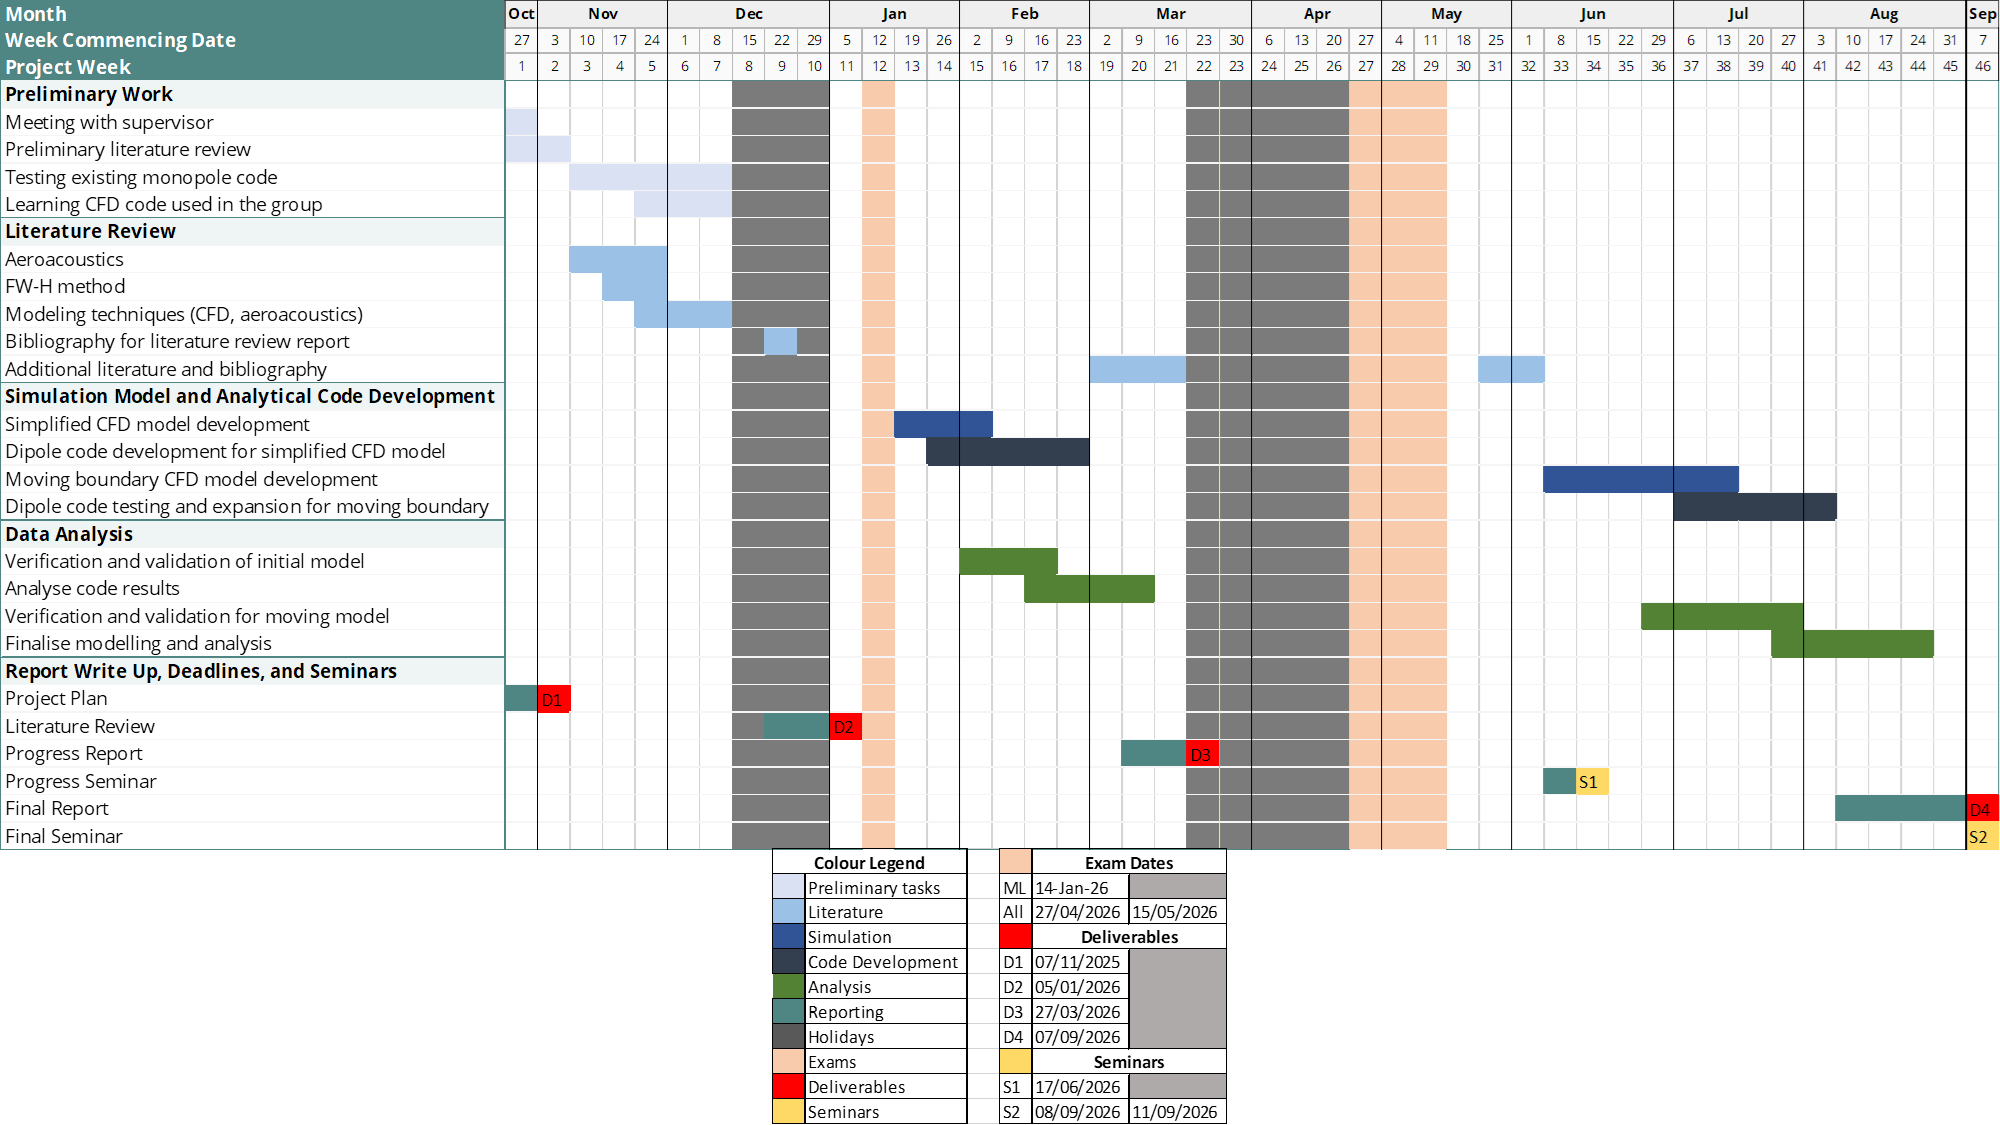
\includegraphics[width=1\linewidth]{fig_past_reports/gantt_chart.png}
    \caption{Gantt Chart of the research project}
    \label{fig:GC}
\end{figure}
\chapter{Literature Review} \label{sec:litrev}

Predicting open rotor noise requires solving the inhomogeneous wave equation. The Ffowcs Williams-Hawkings (FW-H) equation provides the standard analytical framework for this process \cite{Dowling1983}. In this project, the permeable surface, retarded-time formulation is utilised \cite{FfowcsWilliams1969, Brentner1997, Najafi-Yazdi2011}. This formulation was chosen as it captures quadrupole noise sources (from nonlinearities such as shocks and turbulence) via surface integration, provided the control surface fully encapsulates the nonlinearities \cite{Morgans2004}. Therefore, this avoids the computationally expensive volume integrals which is prohibitive to noise prediction. The full expansion of this permeable surface formulation is presented in Appendix \ref{app:fwh_expansion}.

Analytical approaches for monopole sources have been validated in previous work by Char and Thomas \cite{TingChar2024, Thomas2012}; however, expansion into dipoles requires further validation. Monopoles or thickness sources are sounds that are equivalent to mass supply, described as the following,

\begin{equation}
    \Box^2p'(\bm{x},t) = \frac{\partial}{\partial t} (Q(t) \delta(\bm{x} - y(t)))
    \label{eq:monopole_def}
\end{equation}

Convolving the above with the Green's function in 3D free-space gives the following,

\begin{equation}
    p'(\bm{x}, t)= \frac{\partial}{\partial t} \left[ \frac{Q(\tau)}{4\pi r (1-M_r)}\right]_{\tau*}
    \label{eq:monopole_convolved}
\end{equation}

which will be the description of the monopole used throughout this report.

Dipoles or loading sources are sounds due to forces acting on the fluid, equivalent to body forces and momentum supply. It is also equivalent to two equal monopoles with opposite signs at a distance tending to zero. The dipole is described as the following,

\begin{equation}
    p'(\bm{x}, t)=-\frac{\partial}{\partial x_i} \left[\frac{f_i(\tau)}{4\pi r(1-M_r)}\right]_{\tau *}
    \label{eq:dipole_convolved}
\end{equation}

It is necessary to validate the analytical code's prediction of phase, amplitude, and directivity patterns against a known theoretical source before using it to predict noise from CFD data.

\begin{figure}[H]
    \centering
    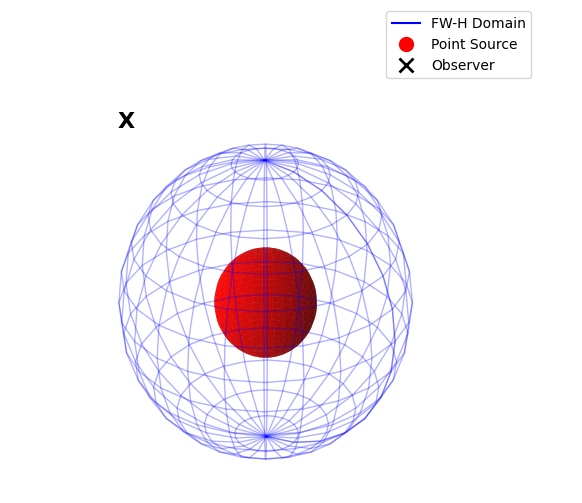
\includegraphics[width=0.9\linewidth]{fig_past_reports/fwh_domain_observer.png}
    \caption{Hybrid domain illustration}
    \label{fig:domain}
\end{figure}

Following this work, CFD will be used as an input to the FW-H code to form a hybrid computational-analytical method, \cite{Kritikos2012, Morgans2004, Thomas2012, Sharma2013}. The Unsteady Reynolds Averaged Navier-Stokes (URANS) framework will be used as it proves effective despite its limitation in capturing high frequency noise from turbulent structures \cite{Fan2025, Mohan2025} from other frameworks such as Detached Eddy Simulation (DES) \cite{Spalart2009} or Large Eddy Simulations (LES). However, for the purpose and limited timeline of this project, URANS is considered sufficient. The point source illustrated in Figure \ref{fig:domain} will later be replaced by the CFD domain.
% The Detached Eddy Simulation (DES) can efficiently resolve noise-emitting turbulent structures \cite{Spalart2009, Fan2025}, as it balances the accuracy of Large Eddy Simulation (LES) in detached flow regions with the lower computational cost of URANS in attached boundary layers. This hybrid DES-FW-H approach will provide a computationally efficient, discrete volumetric source data required for the permeable surface integration.
\clearpage
\chapter{Analytical Derivation of Point Sound Sources} \label{sec:derivations}

In this chapter, the derivations for density, pressure, and velocity perturbation components are described for monopole and dipole sources. These are used to validate the numerical integration of the FW-H code. By comparing the numerical output against the analytical solutions, the code's capability can be validated. For density specifically, the expression is,

\begin{equation}
    \rho'=\frac{p'}{c^2}
    \label{eq:density}
\end{equation}

Which is valid for both monopole and dipole since there is no viscosity nor entropy generation. For pressure, generally the approach would be to convolve the pressure description for  either sources with the Green's function in 3D free-space (Appendix~\ref{app:GF}), described as

\begin{equation}
    G=\frac{\delta(g(\tau))}{4\pi r}
    \label{eq:GreensFunction}
\end{equation}

where $g(\tau)=t-\tau-\frac{r(\tau)}{c}$ and $r(\tau)=|\bm{x}-y(\tau)|$. 

\section{Analytical Solution for a Monopole} \label{subsec:Analytical Solution for a Monopole}

\subsection{Monopole Pressure Equation} \label{subsubsec:mono_p}
Taking the monopole definition as described in Equation \ref{eq:monopole_convolved}, taking the differentiation using the definitions as described in Appendix~\ref{app:derivatives}, the analytical solution for pressure is obtained,% and using the quotient rule to differentiate each term, is obtained,

% \begin{equation*}
%     p'(\bm{x}, t) = \frac{1}{4\pi} \left[ 
%     \frac{\partial Q(\tau) / \partial \tau}{r(1-M_r)^2} -
%     \frac{Q(\tau) v_r}{r^2 |1-M_r|^2} +
%     \left(
%     - \left(\frac{\partial M}{\partial \tau} \right) \frac{Q(\tau)}{r|1-M_r|^3} +
%     \frac{Q(\tau)c(|M|^2 - M_r^2}{r^2 |1-M_r|^3}
%     \right)
%     \right]_{\tau *}
%     \label{eq:monopole_p_der_step1}
% \end{equation*}

% The second term was algebraically manipulated by multiplying both the numerator and denominator by $1 - M_r$ to establish a common denominator and substitute the velocity in the radiation direction, $v_r$, with the speed of sound term, $c$. Then, using further algebraic manipulation for terms with $r^2(1-M_r)^3$ denominators, the analytical solution for pressure is obtained,

\begin{equation}
    p'(\bm{x}, t) = \frac{1}{4\pi} \left[ 
    \frac{\partial Q(\tau) / \partial \tau}{r(1-M_r)^2} +
    \left(\frac{\partial M}{\partial \tau} \right) \frac{Q(\tau)}{r(1-M_r)^3} +
    \frac{Q(\tau) c (M_r - |M|^2)}{r^2(1-M_r)^3}
    \right]_{\tau*}
    \label{eq:monopole_p_der}
\end{equation}

\subsection{Monopole Velocity Equation} \label{subsubsec:monopole_u}

Using the momentum equation,
\begin{equation}
    \rho_0 \frac{\partial u_i}{\partial t} +
    \rho_0 \left( u_i \frac{\partial u_i}{\partial x_j} \right) =
    -\frac{\partial p}{\partial x_i} +
    \frac{\partial}{\partial x_j} \left(
    \mu \left(\frac{\partial u_i}{\partial x_j} + \frac{\partial u_j}{\partial x_i} \right)
    \right)
    \label{eq:momentum_eq}
\end{equation}

Assuming the flow has no mean flow and is inviscid, substituting the monopole definition into the pressure term, and convolving with Green's function to replace $\partial/\partial x_i$ with $\partial/\partial t$, %the solution for velocity is obtained, %the second terms of both left- and right-hand are zero. Defining the pressure gradient by defining the pressure as monopole pressure definition,

% \begin{equation*}
%     - \frac{\partial p}{\partial x_i} =
%     \frac{\partial}{\partial x_i} \frac{\partial}{\partial t} \left[
%     \frac{Q(\tau)}{4\pi r (1-M_r)}
%     \right]_{\tau*}
% \end{equation*}

% and cancelling the unsteady term from both sides gives the following for the momentum equation,

% % \begin{equation*}
% %     \rho_0 \frac{\partial u_i}{\partial t} =
% %     \frac{\partial}{\partial x_i} \frac{\partial}{\partial t} \left[
% %     \frac{Q(\tau)}{4\pi r (1-M_r)}
% %     \right]_{\tau*}
% % \end{equation*}

% % cancelling the unsteady term from both sides leaves,

% \begin{equation}
%     u_i = \frac{1}{\rho_0} \frac{\partial}{\partial x_i} \left[ 
%     \frac{Q(\tau)}{4\pi r (1-M_r)}
%     \right]_{\tau *}
%     \label{eq:monopole_spatial_derivative}
% \end{equation}

% Convolving with Green's function in free 3D-space is done to replace the spatial derivative into a temporal derivative,

% \begin{equation*}
%     p'(\bm{x}, t) = \frac{\partial}{\partial x_i} (Q_i \star G) =
%     - \frac{\partial}{\partial t} \left( 
%     Q_i \star \frac{x_iG}{c|\bm{x}|}
%     \right) -
%     Q_i \star \frac{x_i G}{|\bm{x}|^2}
%     \label{eq:convolve_monopole}
% \end{equation*}

% which has the same form as the integral shown in Appendix \ref{app:derivatives}, Equation \ref{eq:C5}. Substituting the monopole source terms into $Q_i$, and converting to retarded time using the equation found in Appendix \ref{app:ddx_replace} Equation \ref{eq:retarded_time_def}, gives,

% \begin{equation*}
%     \frac{\partial}{\partial x_i} \left[ 
%     \frac{Q(\tau)}{4\pi r (1-M_r)}
%     \right]_{\tau*}
%     = \frac{1}{1-M_r} \frac{\partial}{\partial\tau} \left[ 
%     \frac{Q(\tau)r_i}{4\pi c \bm{r}^2 (1-M_r)^2}
%     \right]_{\tau *}
%     + \left[ 
%     \frac{Q(\tau)r_i}{4 \pi r^3 (1-M_r)}
%     \right]_{\tau*}
%     \label{eq:monopole_velocity_underived}
% \end{equation*}

% which can then be solved analytically to give the solution for velocity,

\begin{equation}
    \begin{split}
    u_i' 
    &= \frac{1}{4\pi\rho_0} \Bigg[ \frac{(\partial Q(\tau)/\partial \tau)r_i}{c r^2(1 - M_r)^2} 
    + \frac{Q(\tau)r_i}{r^3(1-M_r)^3}
    + \left(\frac{dM}{d\tau} \right) \frac{Q(\tau)r_i}{cr^2(1-M_r)^3} \\
    &\phantom{= \frac{1}{4\pi\rho_0}
    \Bigg[} + \frac{Q(\tau)M^2r_i}{r^3(1-M_r)^3}
    - \frac{Q(\tau)M_i}{r^2(1-M_r)^2}
    \Bigg]_{\tau*}
    \end{split}
    \label{eq:monopole_velocity}
\end{equation}
\input{sections/04_Dipole_Derivations}
\chapter{Analytical and Numerical Results Validation} \label{sec:validation}

\section{Description of Validation Process} \label{subsec:validation_description}
To compare the accuracy of the derivations described in Chapter \ref{sec:derivations}, several test cases are used to model a point sound source and an observer. This section describes the test cases used and the validations. Figure \ref{fig:fwh_validation} below illustrates the framework used for validation. 

\begin{figure}[H]
    \centering
    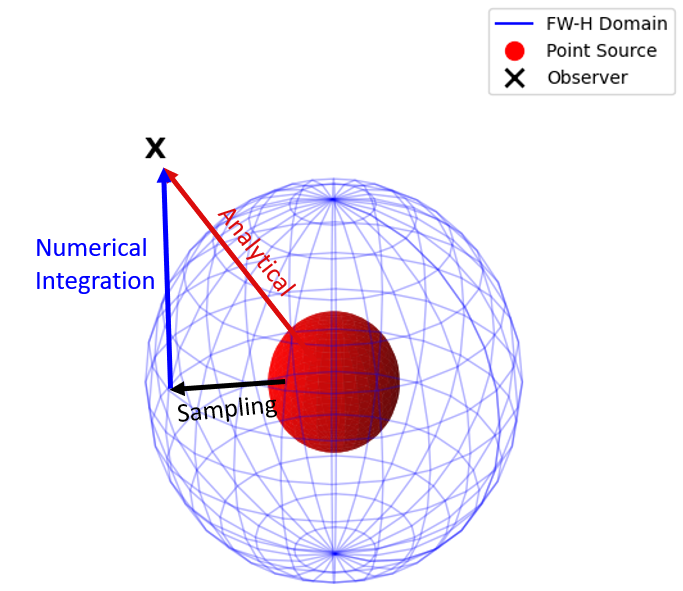
\includegraphics[width=0.5\linewidth]{fig_monopole/fwh_domain_observer_arrows.png}
    \caption{Code validation framework}
    \label{fig:fwh_validation}
\end{figure}

The numerical code samples the source to the permeable boundary (black arrow), followed by surface integration of pressure to calculate the acoustic pressure at the observer (blue arrow). Analytical pressure is calculated directly from the source to the observer (red arrow).

\subsection{Test Cases} \label{subsubsec:test_cases}
In all test cases, the point source is prescribed with strength $Q(\tau)=\sin{(10\tau)}$, from a starting point at the origin, $\left[0,0,0\right]$. Speed of sound $c$ and freestream density $\rho_0$ are set to $340m/s$ and $1.2 kg/m^3$, respectively. The observer's location depends on the case. A control surface surrounding the source are prescribed with a radius $r$. 

These following are based on the work of Char \cite{TingChar2024} and are extended for dipoles:

\begin{itemize}
    \item Stationary and co-translating point source and observer. This test case is used as a baseline to test the overall prediction of the zero relative motion between point source and observer. The tests will also demonstrate the similarity between the two cases. 
    
    \begin{figure}[H]
        \begin{subfigure}[b]{0.495\textwidth}
            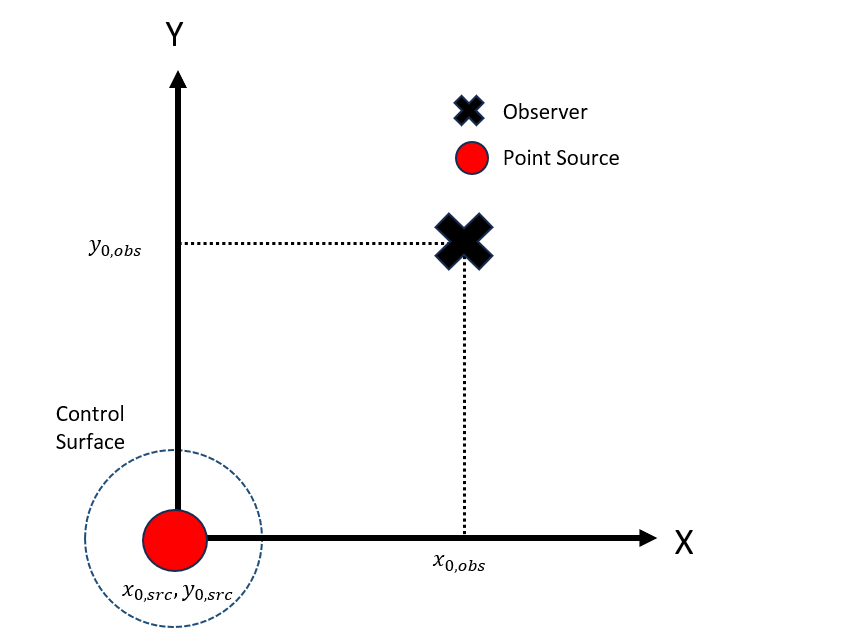
\includegraphics[width=\textwidth]{fig_test_cases/stationary_stationary.png}
            \caption{}
            \label{fig:testcase_ss}
        \end{subfigure}
        \hfill
        \begin{subfigure}[b]{0.495\textwidth}
            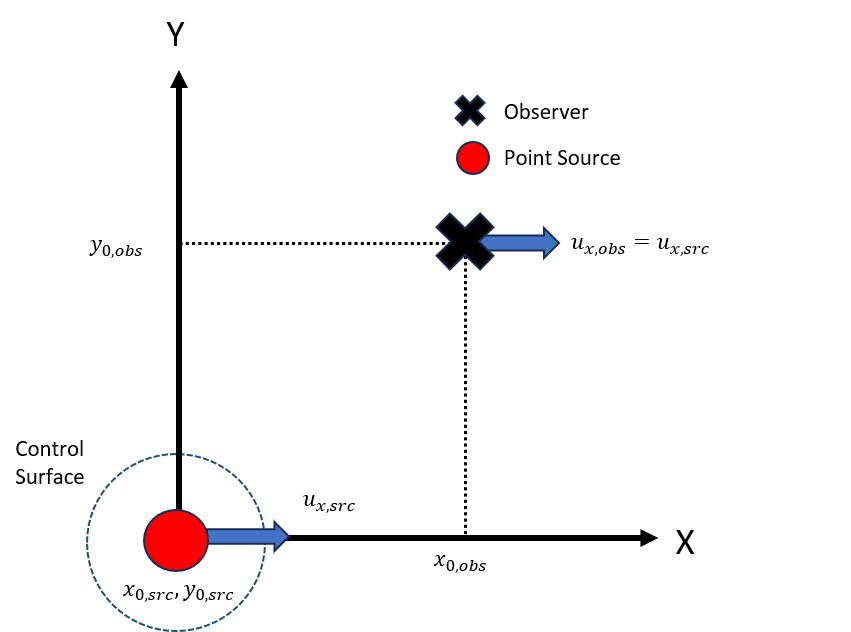
\includegraphics[width=\textwidth]{fig_test_cases/translating_translating.png}
            \caption{}
            \label{fig:testcase_tt}
        \end{subfigure}
        \caption{\centering Illustration of, a) stationary point source and observer, and b) co-translating point source and observer cases}
        \label{fig:testcase_ss_tt}
    \end{figure}
    
    \item Translating point source and stationary observer. This test case demonstrates the prediction with cases of non-zero relative motion between point source and observer, and thus shows the limitations of some of the derivations.
    
    \begin{figure}[H]
        \centering
        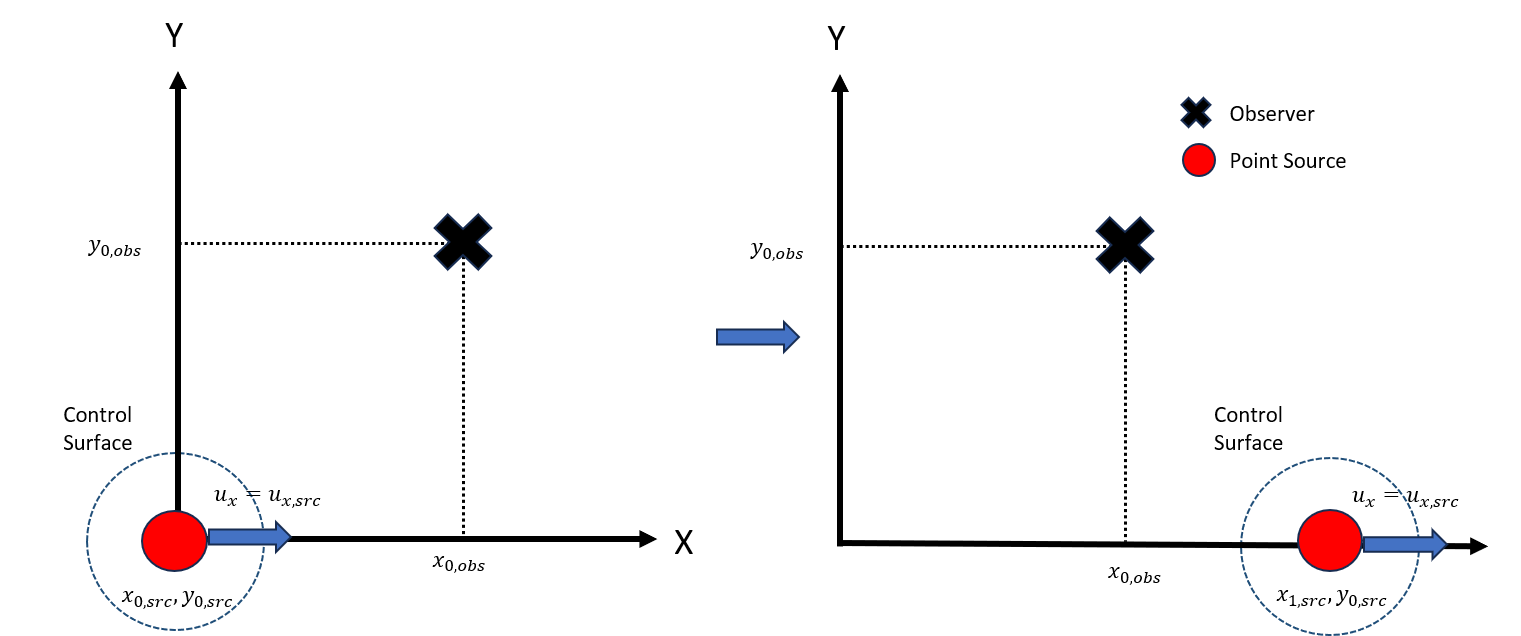
\includegraphics[width=1\linewidth]{fig_test_cases/translating_stationary.png}
        \caption{Illustration of translating point source and stationary observer cases}
        \label{fig:testcase_ts}
    \end{figure}
    
\end{itemize}

Any error are then be quantified using the following,

\begin{equation}
    Error = \frac{\Sigma_j(p_{j,ref} - p_{j,num})^2}{\Sigma_j(p^j_{ref})^2} 
    \label{eq:error}
\end{equation}

\clearpage
% where the subscripts $j$, $ref$, and $num$ are the $j$-th index, reference analytical values, and the numerical integration results, respectively. 

\section{Monopole Validation and Sensitivity Study} \label{subsec:monopole_validation}
The first investigation are of monopole with stationary, as well as co-translating source and observer. This gives a baseline sensitivity of different control surface grid resolutions and time step sizing. The radius of the control surface is set to $1m$, and the observer is located at $[50,50,0]$. In the the co-translation case, the points are translating at $150m/s$ along the x-direction.

For grid sensitivity, the control surface is discretised with $40 \times 40$, $15 \times 15$, and $5\times5$ grids and the time step size is set to $dt=0.005s$. Conversely, for the time step sizing test, the grids are set to $40\times40$ resolution while the time steps are sized to $dt=0.005s$, $dt=0.025s$, and $dt=0.125s$, which correspond to $200 Hz$, $40 H$z, and $8 Hz$ sampling frequencies, respectively.

\begin{figure}[H]
    \centering
    \begin{subfigure}[b]{0.495\textwidth}
        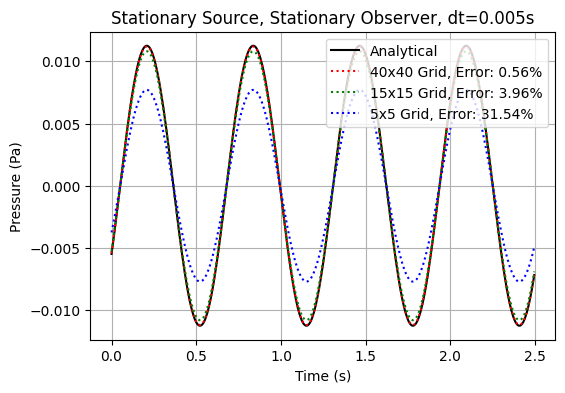
\includegraphics[width=\textwidth]{fig_monopole/monopole_stationary_dx.png}
        \caption{}
        \label{fig:monopole_ss_dx}
    \end{subfigure}
    \hfill
    \begin{subfigure}[b]{0.495\textwidth}
        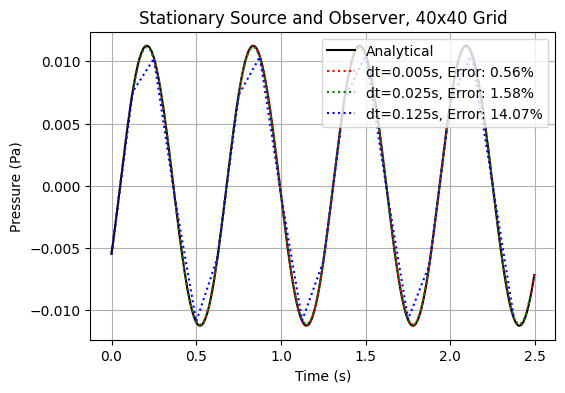
\includegraphics[width=\textwidth]{fig_monopole/monopole_stationary_dt.png}
        \caption{}
        \label{fig:monopole_ss_dt}
    \end{subfigure}

    \vspace{0.25cm}

    \begin{subfigure}[b]{0.495\textwidth}
        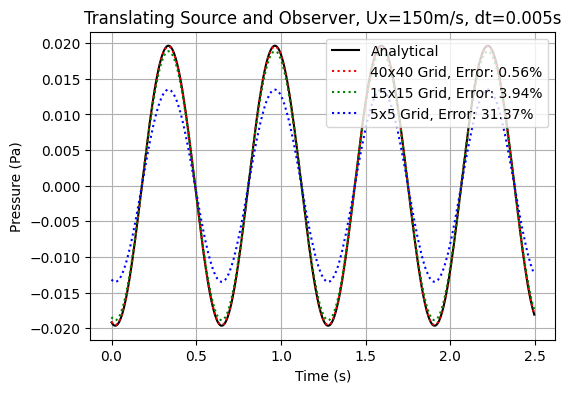
\includegraphics[width=\textwidth]{fig_monopole/monopole_moving_so_dx.png}
        \caption{}
        \label{fig:monopole_tt_dx}
    \end{subfigure}
    \hfill
        \begin{subfigure}[b]{0.495\textwidth}
        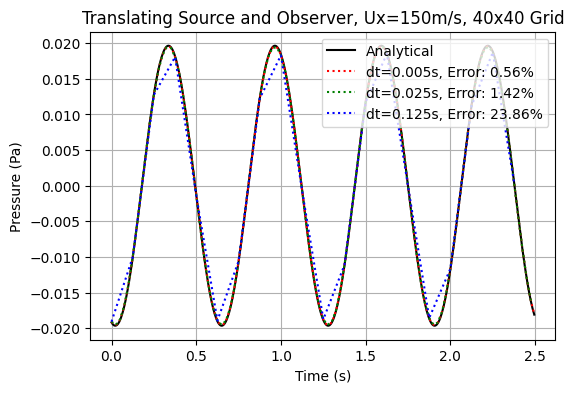
\includegraphics[width=\textwidth]{fig_monopole/monopole_moving_so_dt.png}
        \caption{}
        \label{fig:monopole_tt_dt}
    \end{subfigure}

    \caption[Stationary and zero co-translating monopole test cases]{\centering Stationary and co-translating monopole test cases, a) stationary with varied grid sizing, and b) stationary with varied time-stepping sizing, c) co-translating with varied grid sizing, and d) co-translating  with varied time-stepping sizing}
    \label{fig:monopole_zero_relative}
\end{figure}

For the relative motion case, the grid and time-stepping sensitivity set ups remain the same. The cases differ by translating only the source at $150m/s$ along the x-axis, while the observer remains stationary.

\begin{figure}[H]
    \begin{subfigure}[b]{0.495\textwidth}
        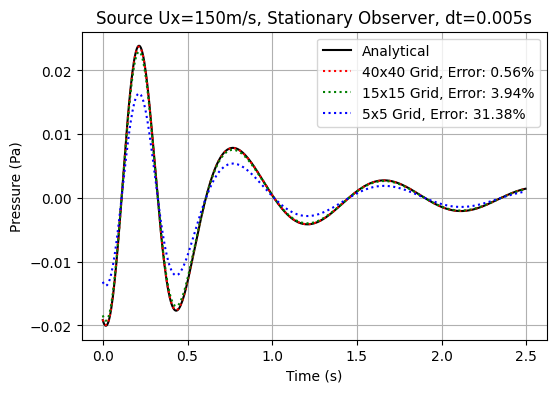
\includegraphics[width=\textwidth]{fig_monopole/monopole_moving_s_dx.png}
        \caption{}
        \label{fig:monopole_ts_dx}
    \end{subfigure}
    \hfill
    \begin{subfigure}[b]{0.495\textwidth}
        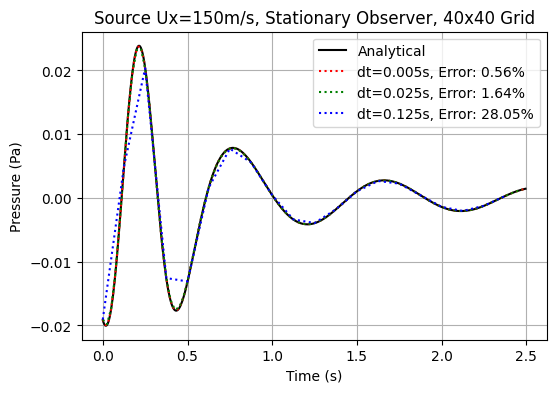
\includegraphics[width=\textwidth]{fig_monopole/monopole_moving_s_dt.png}
        \caption{}
        \label{fig:monopole_ts_dt}
    \end{subfigure}
    \caption[Translating monopole with stationary observer test case]{\centering Translating monopole with stationary observer test case, a) with varied grid sizing, and b) with varied time-step sizing}
    \label{fig:monopole_relative}
\end{figure}

Comparing the first two cases (Figure \ref{fig:monopole_zero_relative}) shows a distinction in amplitude and phase, despite both scenarios having zero relative Mach number ($M_r=0$). In the co-translating case, the source moves through the quiescent fluid medium, which causes a phase shift of $\sim\pi/2$ and pressure increase due to the convective term. Furthermore, the emission distance $r$ in the retarded time, $\tau = t - r/c$, differs from the geometric distance because both points are moving through the medium during the propagation time. The third case demonstrates the effect of relative Mach number. In Figure \ref{fig:monopole_relative} the Doppler effect causes the acoustic frequency and pressure amplitude received by the observer to increase as the source approaches ($0\leq t\leq 0.33s$), and decrease as it moves away ($t>0.33s$).

In the grid resolution comparisons, while the finest resolution of $40\times40$ has very good agreement with the analytical solutions at less than $1\%$ error in all cases, the errors progressively increase to $\sim4\%$ and $\sim 30\%$, for coarser resolutions. The plots show at lower resolution, the numerical results could not capture the peaks and troughs of the harmonic wave, causing dissipation. Given the acoustic wavelength is $\sim214m$ (from the prescribed frequency and speed of sound values), the coarsest grid has an arc distance between two nodes of 1.25 meters. The errors shown in the grid sensitivities are mainly due to geometric error of the spherical domain, rather than the grids not being able to capture the wavelengths. This shows that this grid resolution is sufficient given the input and control surface radius.

The time step sensitivity study exhibits similar trends. The $dt=0.005s$ and $dt=0.025s$ sizes yield errors at less than $1\%$ and $2\%$, respectively. However, largest time-step size of $dt=0.125s$ (an $8Hz$ sampling frequency), is insufficient to capture the input acoustic frequency of $10rad/s$ or $\sim1.6Hz$, as it can only sample at five times the input. This can be seen in the lags in the plots as the numerical solution attempted to keep up with the wave.
\input{sections/06_Dipole_Validations}
\input{sections/07_directivity}
\chapter{Discussion} \label{sec:discussion}

The FW-H code has been validated for monopole sources. The sensitivity studies confirmed that spatial discretisation affects the geometric accuracy of the spherical control surface. Similarly, temporal discretization must be fine enough to prevent the clipping of harmonic peaks for frequencies of interest.

The co-translating monopole case presented an interesting point. Despite having a zero relative Mach number ($M_r = 0$), the motion of the source through the quiescent fluid causes a phase shift of $\sim\pi/2$ compared to the stationary case. This is due to the proportionality of the convective term to the source $Q(\tau)$ rather than its derivative $\partial Q/\partial\tau$. Furthermore, the emission distance $r$ affects the retarded time calculation ($\tau = t - r/c$) as the wave moves between the translating points.

However, the dipole validation highlighted the limitations of explicitly deriving velocity terms. The results provide good agreement only when their assumptions are met. Assuming an analytical solution by a zero relative Mach number removes the $(1-M_r)$ factor, causing the analytical solution incapable of predicting moving sources. Similarly, the plane wave assumption fails with near-field control surface. The dual-monopole method alleviates these limitations by superimposing two physical monopoles, which preserves the convective terms without requiring explicit integration.

The limitations of the analytical boundary conditions are also shown in the plane wave test case (Figure \ref{fig:dual_far_valid}). The noticeably lower pressure amplitude  during the source's approach is an error due to imposing a static $x$-direction contribution on the dipole. As the source translates far downstream, the radiation vector creates an asymptote with the $x$-axis, such that the numerical and analytical results eventually match.

As briefly mentioned for the dual monopole results in sub-subchapter \ref{subsubsec:dipole_dual_monopole_validation}, the dual monopole approach shows numerical artefacts as the source moves away from the observer (Figure \ref{fig:dual_far_invalid}). This is likely due to a floating-point truncation error in the numerical code, as it lacks the required prevision for such small perturbation values. As most aeroacoustics codes solve in double-precision, the code needs to be updated to resolve these small perturbations for multiple sources.

To improve the accuracy of the dipole validation, the static $x$-direction constraint could be resolved by dynamically vectoring the dipole orientation normal to the control surface relative to the observer. Furthermore, the dipole source $f_i$ definition could be improved by using a non-stationary monopole equation to preserve the Doppler factor. Given these identified limitations in the analytical baseline, further studies to validate the dipoles are required before using the code to process CFD data.
\chapter{Conclusions} \label{sec:conclusions}

A Ffowcs Williams-Hawkings (FW-H) acoustic code has been analytically validated. The numerical integration is accurate, matching analytical derivations for stationary and moving monopole sources with less than $1\%$ error under sufficient grid and temporal resolution.

For dipole sources, the explicit analytical derivations were shown to break down when subjected to non-zero relative motion or near-field control surfaces. To bypass these limitations, a dual-monopole approach was implemented, proving to be a good test case to demonstrate dipoles. While the numerical integration is mathematically sound, further refinement of the dipole analytical validation method is required. Once complete, the code will be integrated with URANS CFD for open rotor noise prediction.
\chapter{Future Work}
With the FW-H solver validated with some limitations, the project moves to the hybrid analytical-computational framework. The next part of the work include:

\begin{itemize}
    \item Validation refinements for dipoles (e.g., using non-stationary monopole as the source term, dynamic vector calculations) to reduce errors.
    \item Updating the numerical FW-H integration code to use double-precision floating-point arithmetic.
    \item Development and validation of a baseline URANS-FW-H hybrid model.
    \item Using the validated URANS-FW-H approach to predict open rotor noise.
\end{itemize}

%TC:ignore
% ------ Gen AI -------
\clearpage
\chapter*{Review of Generative AI Use}

Generative AI (Google Gemini 3 Pro) has been used in augmenting the research and writing of this report. The usage of which are in helping with LaTeX formatting, formalising some English language uses, mathematical derivations, and checking for programming errors or bugs. The following are prompt examples used on the above main usages:

\begin{itemize}
    \item "Help me format this LaTeX document using the structure abstract, table of contents, nomenclature, intro, lit review, derivations, validations, discussion, conclusions, future work, appendices. The word count should only include the main content (from intro to future work).
    \item "Help me rephrase these two sentences and bridge between them"
    \item "In deriving the velocity equation for the dipole, as the explicit integral of the convolution between the right hand side term and Green's function is unviable, what would be the implications of assuming that r is a constant value, such that some integrations of the F/(1-M\_r) term can be done? If this is solved in the retarded time, the denominator is cancelled, so I can integrate F directly, correct?
    \item "As the dual monopole method requires introducing an additional point source, which the code had not considered initially, help me to put an additional point monopole in the sample\_properties subroutine in Fortran. As per the derivations, I need to separate the two by a distance delta, which I think can just be calculated as 0.01/k so it dynamically changes if any parameters are changed in the future.
\end{itemize}

The result of the first two examples being in the formatting of this report and some of the sentences within. None of the result sentences are directly copied from the tool, and instead are rephrased in the author's own words to reflect the author's understanding of the topic. The third prompt helped the author in deriving the mathematical parts presented in this report; of which the results are checked and verified via textbooks and during meetings with supervisors. The fourth prompt example returned Fortran codes that are used for the analytical solutions. These solutions tend to come with bugs which the author fixed independently.

In conclusion, all text-based outputs given by the Generative AI were checked, reworded, and edited to be based on the author's understanding of the topic and to avoid plagiarism. Outputs that are technical are verified by textbooks and discussions with supervisors to ensure the accuracy of the results and limitations of the assumptions.

% ------ APPENDICES -------
\clearpage
\begin{appendices}
\numberwithin{equation}{chapter}

% !TEX root = ../main.tex

\chapter{Research Project Gantt Chart} \label{app:ganttchart}

The following is the Gantt Chart of the current project up to its completion. Some adjustments had to be made along the duration of the project's execution such as CFD-related parts, however, the overall project objectives and milestones remain the same.

\begin{figure}[H]
    \centering
    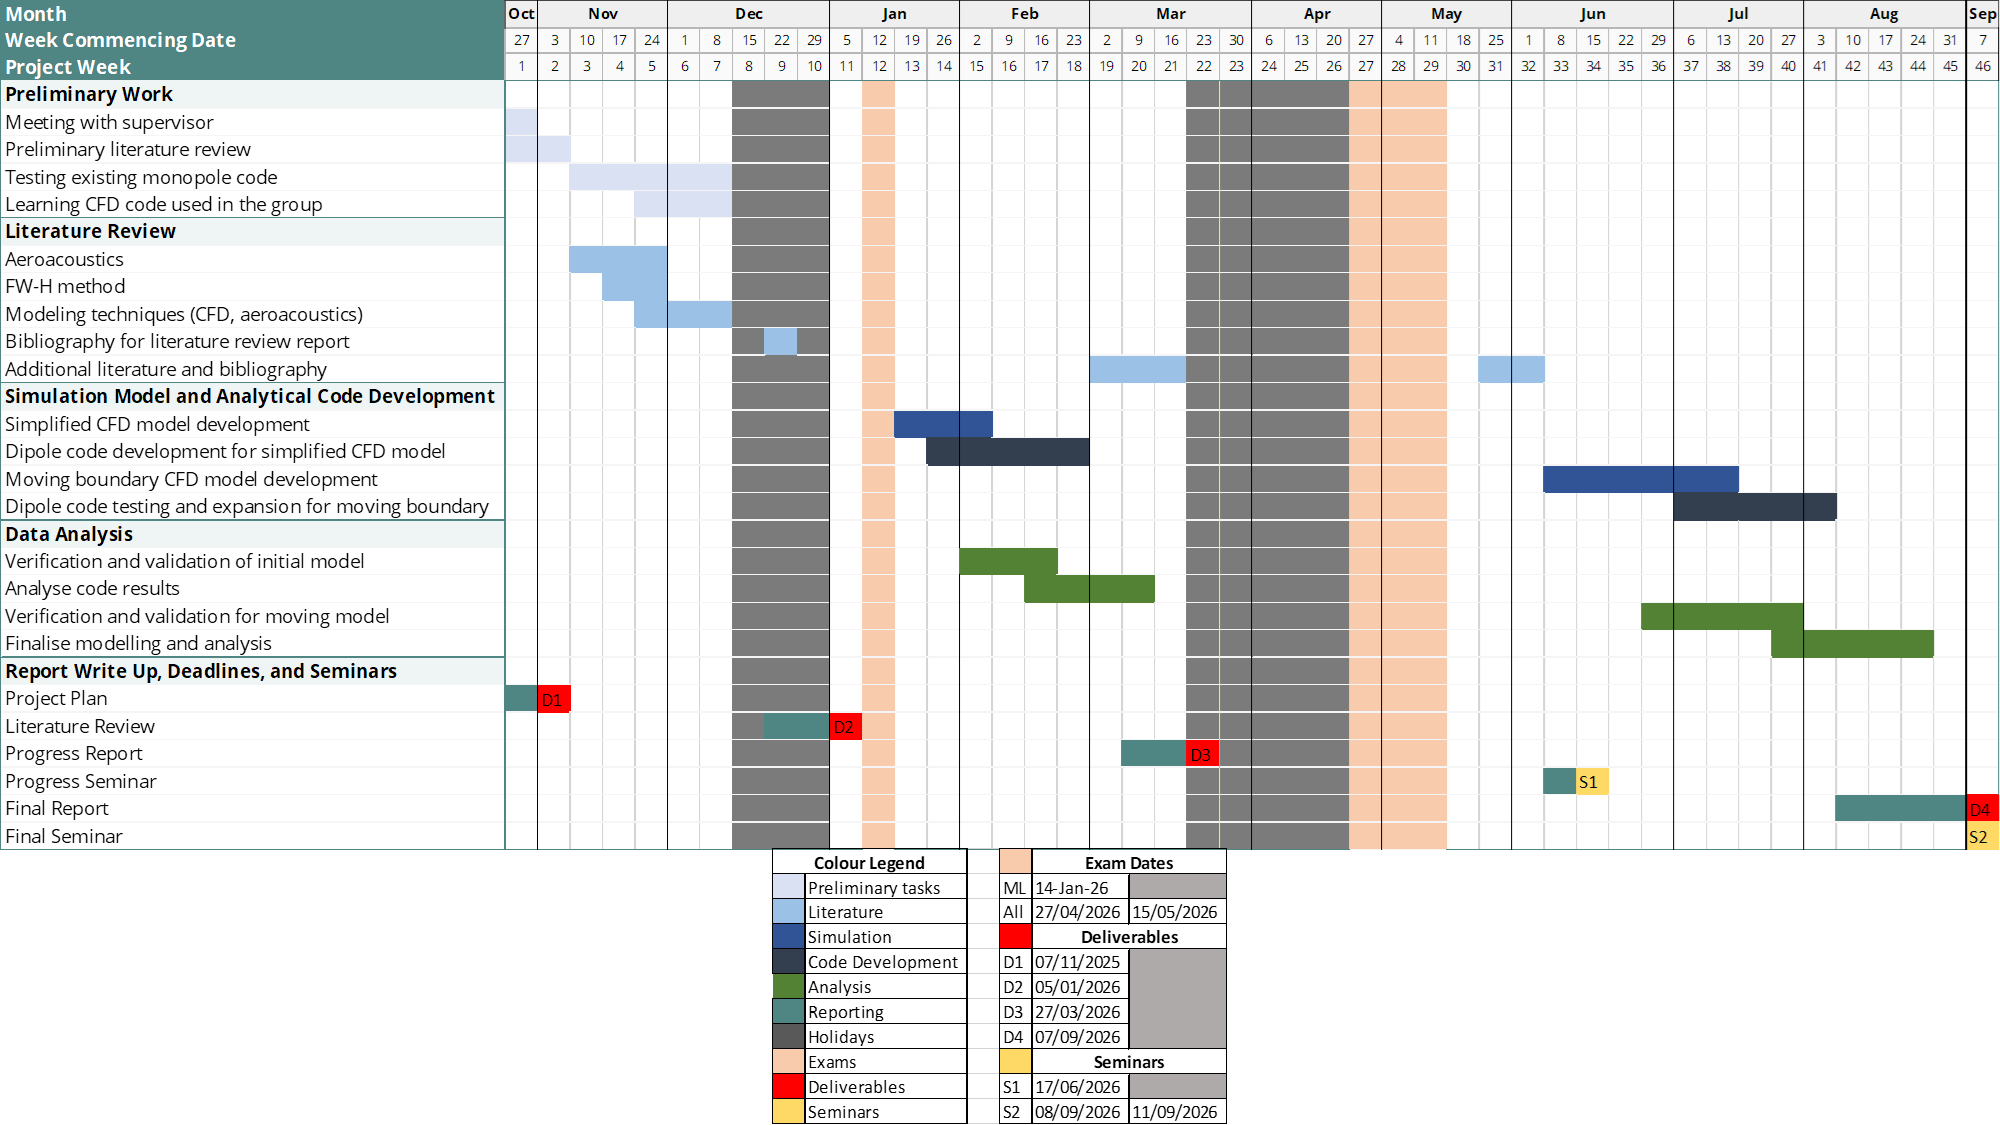
\includegraphics[width=1\linewidth]{fig_past_reports/gantt_chart.png}
    \caption{Gantt Chart of the research project}
    \label{fig:GC}
\end{figure}

\chapter{Variable Derivatives} \label{app:derivatives}

To derive the analytical point sources, a few definition for the derivatives are established.

\begin{equation}
    \left. \frac{\partial r}{\partial \tau} \right|_x =  -v_r
    \label{eq:C1}
\end{equation}

\begin{equation}
    \left. \frac{\partial M_r}{\partial \tau} \right|_x = \left( \frac{\partial M}{\partial \tau} \right)_r +
    \frac{c(M_r^2-|M|^2)}{r}
    \label{eq:C2}
\end{equation}

\begin{equation}
    \left. \frac{\partial |1-M_r|}{\partial\tau} \right|_x = \frac{(1-M_r)}{|1-M_r|}
    \left(
    -\left( \frac{\partial M}{\partial \tau}
    \right)_r  +
    \frac{c(|M|^2 - M_r^2}{r}
    \right)
    \label{eq:C3}
\end{equation}

\begin{equation}
    \left. \frac{\partial [Q(\tau)]_{\tau*}}{\partial\tau}\right|_x
    = \left.
    \left[ \frac{1}{1-M_r} \frac{\partial Q(\tau)}{\partial \tau} \right]_x
    \right|_{\tau*}
    \label{eq:C4}
\end{equation}

\begin{equation}
    \left. - \frac{\partial}{\partial x_i}
    \right|_t \int_S [Q_i]_{\tau*} dS =
    \left. \frac{\partial}{\partial t}\right|_x \int_S \left[ \frac{Q_ir_i}{cr}\right]_{\tau*}dS + \int_S \left[ \frac{Q_ir_i}{r^2}\right]_{\tau*}dS
    \label{eq:C5}
\end{equation}

% \chapter{Permeable Surface with Retarded Time Formulation} \label{app:fwh_expansion}

% Given the inhomogeneous wave equation in the integral form of the FW-H equation,
% \begin{equation}
%     \begin{split}
%         \Box^2p'(\bm{x},t) &=
%         \frac{\partial^2}{\partial x_i\partial x_j} \int_{-\infty}^{\infty} \frac{\overline{T_{ij}}\delta(g)J}{4\pi r}d^3\eta d\tau \\
%         &\quad - \frac{\partial}{\partial x_i} \int_{-\infty}^\infty \frac{\left(p_{ij}n_j+\rho u_i (u_n-v_n) \right) \delta(f)\delta(g) |\nabla_xf|J}{4\pi r} d^3\eta d\tau \\
%         &\quad + \frac{\partial}{\partial t} \int_{-\infty}^\infty \frac{\left(\rho_0u_n + \rho'(u_n-v_n) \right) \delta(f)\delta(g) |\nabla_xf|J}{4\pi r}d^3\eta d\tau
%     \end{split}
%     \label{eq:FWH}
% \end{equation}

% The first RHS term, the quadrupole, is not dealt with explicitly \cite{Parry1988, Hanson1985} as it is more significant for transonic and supersonic Mach numbers \cite{FfowcsWilliams1969, Ffowcs1969}. By choosing a sufficiently large permeable surface, the quadrupole contributions outside of this surface is negligible,

% \begin{equation}
%     \begin{split}
%         \Box^2p'(\bm{x},t) &=
%         - \frac{\partial}{\partial x_i} \int_{-\infty}^\infty \frac{\left(p_{ij}n_j+\rho u_i (u_n-v_n) \right) \delta(f)\delta(g) |\nabla_xf|J}{4\pi r} d^3\eta d\tau \\
%         &\quad + \frac{\partial}{\partial t} \int_{-\infty}^\infty \frac{\left(\rho_0u_n + \rho'(u_n-v_n) \right) \delta(f)\delta(g) |\nabla_xf|J}{4\pi r}d^3\eta d\tau
%     \end{split}
%     \label{eq:FWH_no_quad}
% \end{equation}

%  Using the notation by di Francescantonio \cite{Francescantonio1997} to simplify the algebra, new variables $U_i$ and $L_i$ are introduced to represent mass and momentum fluxes through the control surface,

% \begin{equation*}
%     U_i=(1-\frac{\rho}{\rho_0})v_i  + \frac{\rho}{\rho_0}u_i \quad     L_i=p_{ij}n_j+pu_i(u_n-v_n)
% \end{equation*}

% Considering an undistorted control surface that translates at a constant and subsonic velocity, the retarded time formulation, as described by Brentner and Farassat \cite{Brentner1998} is,

% \begin{equation}
% \begin{split}
%     p'(\bm{x}, t) &= \frac{1}{4\pi} \int_{S} \left[ \frac{\rho_0 (\dot{U}_n + U_{\hat{n}})}{r(1-M_r)^2} \right]_{\tau^*} dS(\eta) \\
%     &\quad + \frac{1}{4\pi} \int_{S} \left[ \frac{\rho_0 (r(dM/d\tau)_r + c(M_r - |M|^2))}{r^2(1-M_r)^3} \right]_{\tau^*} dS(\eta) \\
%     &\quad + \frac{1}{4\pi c} \int_{S} \left[ \frac{\dot{L}_r}{r(1-M_r)^2} \right]_{\tau^*} dS(\eta) \\
%     &\quad + \frac{1}{4\pi} \int_{S} \left[ \frac{L_r - L_m}{r^2(1-M_r)^2} \right]_{\tau^*} dS(\eta) \\
%     &\quad + \frac{1}{4\pi c} \int_{S} \left[ \frac{L_r(r(dM/d\tau)_r + c(M_r - |M|^2))}{r^2(1-M_r)^3} \right]_{\tau^*} dS(\eta)
% \end{split}
% \label{eq:fwh_full_expansion_ch2}
% \end{equation}

% The retarded time are calculated implicitly via the Newton-Raphson root-finding method. 

\chapter{Green's Function for Wave Equations} \label{app:GF}
Given a wave equation,
\begin{equation*}
    \left(\nabla^2 - \frac{1}{c^2}\frac{\partial^2}{\partial t^2} \right) \psi(\hat{r},t)=-f(\hat{r},t)
\end{equation*}

Green's function of the above equation,
\begin{equation*}
    \left(\nabla^2 - \frac{1}{c^2}\frac{\partial^2}{\partial t^2} \right) G(\hat{r},t |\hat{r'},t')=-\delta(\hat{r'}-\hat{r})\delta(t-t')
\end{equation*}

Let $\hat{r'}=0$ and $t'=0$. Solving for $\nabla^2G$
\begin{equation*}
    \begin{split}
        \nabla^2G(\hat{r},t) &= \frac{1}{r^2}\frac{\partial}{\partial r} \left(r^2 \frac{\partial}{\partial r} \right)G \\
        &\quad =\frac{1}{r} \frac{\partial G}{\partial r} + \frac{1}{r} \left( \frac{\partial G}{\partial r} + r \frac{\partial^2G}{\partial r^2} \right) \\
        &\quad = \frac{1}{r} \frac{\partial^2}{\partial r^2} (rG).
    \end{split}
\end{equation*}

Substituting back to the wave form,
\begin{equation*}
    \nabla^2G - \frac{1}{c^2}\frac{\partial^2}{\partial t^2}G=-\delta(r)\delta(t)
\end{equation*}
\begin{equation*}
    \frac{1}{r}\frac{\partial^2}{\partial r^2}(rG) - \frac{1}{c^2}\frac{1}{r}\frac{\partial^2}{\partial t^2} (rG)=-\delta(r)\delta(t)
\end{equation*}

Factoring the differential terms, it is found that if $r>0$, then the left-hand side term is equal to zero,

\begin{equation}
    \left[\left(\frac{1}{c}\frac{\partial}{\partial t} + \frac{\partial}{\partial r} \right)\left(\frac{1}{c}\frac{\partial}{\partial t} - \frac{\partial}{\partial r} \right) \right](rG)=0
    \label{eq:green_step1}
\end{equation}

Then, let $u=ct-r$ and $v=ct+r$, it will be found that,
\begin{equation*}
    \frac{\partial}{\partial u} = \frac{1}{2} \left(\frac{1}{c}\frac{\partial}{\partial t} -\frac{\partial}{\partial r}\right)
    \quad
    \frac{\partial}{\partial v} = \frac{1}{2} \left(\frac{1}{c}\frac{\partial}{\partial t} +\frac{\partial}{\partial r}\right)
\end{equation*}

Given that $\partial^2(rG)/(\partial u\partial v)=0$, if $rG=g(v)=g_+(ct+r)$ and $rG=g(u)=g_-(ct-r)$, then,

\begin{equation*}
    G=\frac{1}{r}g_{\pm}(ct\pm r)
\end{equation*}
\begin{equation*}
    G(\hat{r},t | \hat{r'},t')=\frac{1}{\hat{r}-\hat{r'}}g_{\pm}(c(t-t') \pm |\hat{r} - \hat{r'}|)
\end{equation*}

Taking $\nabla^2G$ using this definition,
\begin{equation*}
    \begin{split}
        \nabla^2G&=\nabla^2 \left(\frac{1}{r}g_{\pm}(ct\pm r) \right) =\nabla^2 \left(\frac{1}{r}\nabla g_{\pm} + g_{\pm} \nabla \left(\frac{1}{r} \right) \right) \\
        &\quad = - \frac{2}{r^2}\frac{\partial g}{\partial r} + \frac{2}{r^2}\frac{\partial g}{\partial r} + \frac{1}{r}\frac{\partial^2g}{\partial r^2} - 4\pi \delta(r)g
    \end{split}
\end{equation*}

The first two terms of the right-hand side cancel, and moving back to the wave equation format,

\begin{equation}
    \nabla^2G-\frac{1}{c^2}\frac{\partial^2}{\partial t^2}G = -\frac{1}{r} \left(\frac{1}{c^2}\frac{\partial^2}{\partial t^2} - \frac{\partial ^2}{\partial r^2}\right)g_{\pm} - 4\pi \delta(r)g_{\pm}
    \label{eq:green_step2}
\end{equation}

As described in equation \ref{eq:green_step1}, the first term of the right-hand side cancels. Going back to the wave equation,

\begin{equation*}
    \Box^2 \psi(\hat{r},t)=-\delta(\hat{r})\delta(t)=-4\pi \delta(\hat{r})g_{\pm}
\end{equation*}

Therefore, 
\begin{equation}
    \therefore \quad G_{\pm}=\frac{\delta(ct\pm r)}{4\pi r}
    \label{eq:greensfunction_derived}
\end{equation}

\chapter{Replacing \texorpdfstring{$\partial / \partial x_i$}/ Terms} \label{app:ddx_replace}

As the definition of dipoles are that of the spatial derivative of the forcing term convolved with the Green's function in 3D free-space, it is necessary to replace the spatial derivative terms to that of the temporal one to derive using the definitions described in Appendix \ref{app:derivatives}. As the goal is to transform $\textbf{x} \rightarrow \textbf{X}$ and $t\rightarrow\tau$, and the following are true: $\textbf{x}=\textbf{X}$ and $\tau=t-\frac{\textbf{r}}{c}$, then

\begin{equation*}
    \left. \frac{\partial}{\partial x_i} \right|_t = 
    \frac{\partial X_j}{\partial x_i} \frac{\partial}{\partial X_j} + \frac{\partial\tau}{\partial x_i} \frac{\partial}{\partial\tau}=\delta_{ij}\frac{\partial}{\partial X_j} - \frac{r_i}{cr(1-M_r)}\frac{\partial}{\partial\tau}
\end{equation*}

% As stated previously that $\textbf{x}=\textbf{X}$,

\begin{equation}
    \frac{\partial}{\partial x_i} = \frac{\partial}{\partial x_i} - \frac{r_i}{cr(1-M_r)}\frac{\partial}{\partial\tau}
\end{equation}

Similarly for the  time derivative,

\begin{equation*}
    \left. \frac{\partial}{\partial t} \right|_{\textbf{x}} = \frac{\partial X_j}{\partial t} \frac{\partial}{\partial X_j} + \frac{\partial\tau}{\partial t} \frac{\partial}{\partial \tau}
\end{equation*}

Assuming no mean flow, the first term of the right hand side, $\partial X_i/\partial t$ is equal to zero, leaving,

\begin{equation}
    \left. \frac{\partial}{\partial t} \right|_{\textbf{x}} = \frac{1}{1-M_r} \left. \frac{\partial}{\partial \tau} \right|_{\textbf{x}}
    \label{eq:retarded_time_def}
\end{equation}

\chapter{Monopole Velocity Derivations} \label{app:mono_u}
Using the momentum equation, assuming the flow has no mean flow and is inviscid, substituting the monopole definition into the pressure term, the second terms of both left- and right-hand are zero. Defining the pressure gradient by defining the pressure as monopole pressure definition,

\begin{equation*}
    - \frac{\partial p}{\partial x_i} =
    \frac{\partial}{\partial x_i} \frac{\partial}{\partial t} \left[
    \frac{Q(\tau)}{4\pi r (1-M_r)}
    \right]_{\tau*}
\end{equation*}

and cancelling the unsteady term from both sides gives the following for the momentum equation,

% \begin{equation*}
%     \rho_0 \frac{\partial u_i}{\partial t} =
%     \frac{\partial}{\partial x_i} \frac{\partial}{\partial t} \left[
%     \frac{Q(\tau)}{4\pi r (1-M_r)}
%     \right]_{\tau*}
% \end{equation*}

% cancelling the unsteady term from both sides leaves,

\begin{equation}
    u_i = \frac{1}{\rho_0} \frac{\partial}{\partial x_i} \left[ 
    \frac{Q(\tau)}{4\pi r (1-M_r)}
    \right]_{\tau *}
    \label{eq:monopole_spatial_derivative}
\end{equation}

Convolving with Green's function in free 3D-space is done to replace the spatial derivative into a temporal derivative,

\begin{equation*}
    p'(\bm{x}, t) = \frac{\partial}{\partial x_i} (Q_i \star G) =
    - \frac{\partial}{\partial t} \left( 
    Q_i \star \frac{x_iG}{c|\bm{x}|}
    \right) -
    Q_i \star \frac{x_i G}{|\bm{x}|^2}
    \label{eq:convolve_monopole}
\end{equation*}

which has the same form as the integral shown in Appendix \ref{app:derivatives}, Equation \ref{eq:C5}. Substituting the monopole source terms into $Q_i$, and converting to retarded time using the equation found in Appendix \ref{app:ddx_replace} Equation \ref{eq:retarded_time_def}, gives,

\begin{equation*}
    \frac{\partial}{\partial x_i} \left[ 
    \frac{Q(\tau)}{4\pi r (1-M_r)}
    \right]_{\tau*}
    = \frac{1}{1-M_r} \frac{\partial}{\partial\tau} \left[ 
    \frac{Q(\tau)r_i}{4\pi c \bm{r}^2 (1-M_r)^2}
    \right]_{\tau *}
    + \left[ 
    \frac{Q(\tau)r_i}{4 \pi r^3 (1-M_r)}
    \right]_{\tau*}
    \label{eq:monopole_velocity_underived}
\end{equation*}

which can then be solved analytically to give the solution for velocity,

\begin{equation}
    \begin{split}
    u_i 
    &= \frac{1}{4\pi\rho_0} \Bigg[ \frac{(\partial Q(\tau)/\partial \tau)r_i}{c r^2(1 - M_r)^2} 
    + \frac{Q(\tau)r_i}{r^3(1-M_r)^3}
    + \left(\frac{dM}{d\tau} \right) \frac{Q(\tau)r_i}{cr^2(1-M_r)^3} \\
    &\phantom{= \frac{1}{4\pi\rho_0}
    \Bigg[} - \frac{Q(\tau)M^2r_i}{r^3(1-M_r)^3}
    - \frac{Q(\tau)M_i}{r^2(1-M_r)^2}
    \Bigg]_{\tau*}
    \end{split}
    % \label{eq:monopole_velocity}
\end{equation}


\chapter{Dipole Velocity: Stationary Assumption} \label{app:zeroMach}
Defining pressure gradient from the momentum equation and dipole definition,

\begin{equation*}
    -\frac{\partial p}{\partial x_i} = 
    \frac{\partial^2}{\partial x_i \partial x_j} \left[ 
    \frac{f_i(\tau)}{4\pi r (1-M_r)}
    \right]_{\tau*}
\end{equation*}

Going back to momentum equation, the velocity is,

\begin{equation*}
    u_i = \frac{1}{4\pi\rho_0} \frac{\partial^2}{\partial x_i \partial x_j} \int_{-\infty}^t \frac{f_i(\tau)}{r(1-M_r)}dt
\end{equation*}

assuming $dr/dt=0$ and $M_r=0$, letting $F_i(\tau) = \int f_i(\tau) d\tau \implies f_i(\tau) = \dot{F}_i(\tau)$, and changing to integrating with respect to $\tau$, this simplifies the integrand to,

\begin{equation*}
    u_i = \frac{1}{4\pi r\rho_0} \frac{\partial^2}{\partial x_i \partial x_j} \int_{-\infty}^t {f_i(\tau)}d\tau
\end{equation*}

Taking the integral,

\begin{equation*}
    u_i = \frac{1}{4\pi r\rho_0} \frac{\partial^2}{\partial x_i \partial x_j} \int_{-\infty}^t {f_i(\tau)}d\tau
    =
    \frac{1}{4\pi r\rho_0} \frac{\partial^2}{\partial x_i \partial x_j} \left[F_i(\tau-r/c)
    \right]
\end{equation*}

Hence, the analytical solution for velocity that is valid for cases of zero relative Mach number between the source and observer for near- and far-field,

\begin{equation}
    u_i=\frac{1}{4\pi\rho_0} \left( 
    \frac{F_j(3n_in_j-\delta_{ij})}{r^3} +
    \frac{f_j(3n_in_j - \delta_{ij})}{cr^2} +
    \frac{\dot{f_j}(n_in_j)}{c^2r}
    \right)
    % \label{eq:dipole_u1}
\end{equation}

\chapter{Dipole Velocity: Plane Wave Assumption} \label{app:planeWave}

Given the plane wave,
\begin{equation}
    p'(\bm{x},t)=\frac{g(t-r/c)}{r}
    \label{eq:plane_wave_def}
\end{equation}

Taking the pressure gradient,

\begin{equation*}
    \frac{\partial p'}{\partial x_i} = 
    \left[\frac{\partial}{\partial x_i}\frac{1}{r}g \right] +
    \frac{1}{r} \left[ \frac{\partial}{\partial x_i}g 
    \right]
\end{equation*}

where the first and second terms correspond to the near- and far-field, respectively. The plane wave is valid only in the far-field, and taking the time derivative yields,

\begin{equation*}
    \frac{\partial p'}{\partial t} = \left[ 
    \frac{\partial}{\partial t} \frac{g}{r}
    \right]
    = \frac{1}{r} \frac{\partial}{\partial t} g(\tau) - g(\tau) \frac{v_r}{r^2}
\end{equation*}

In the far-field, $\frac{1}{r}\frac{\partial}{\partial t}g(\tau) \gg g(\tau) \frac{v_r}{r^2}$, simplifying the expression to,

\begin{equation*}
    \frac{\partial p'}{\partial t} \approx \frac{1}{r}\frac{\partial}{\partial t} g(\tau)
\end{equation*}

which gives the following expression,

\begin{equation*}
    \frac{\partial p'}{\partial x_i} = -\frac{n_i}{c} \frac{\partial p'}{\partial t}
\end{equation*}

substituting into the momentum equation provides the velocity equation for the plane wave,

\begin{equation}
    u_i = \frac{n_i}{\rho_0c}p'(\bm{x},t)
    % \label{eq:dipole_u2}
\end{equation}
\end{appendices}

% ------ REFERENCES --------
\clearpage
\bibliographystyle{ieeetr}
\bibliography{references}
%TC:endignore

\end{document}